\subsection{Investigative Techniques}
The following techniques were employed for the implementation of ThermoSight:

\subsubsection*{Research Techniques}
A combination of descriptive and experimental research approaches were utilized to investigate challenges in thermal image classification, Vision Transformer adaptation, and real-time deployment for civil‐engineering inspections. These techniques are detailed in Table \ref{tab:ts_research_techniques}:

\begin{table}[H]
	\centering
	\fontsize{10}{12}\selectfont
	\caption{Research Techniques}
	\label{tab:ts_research_techniques}
	\begin{tabularx}{\textwidth}{|l|X|X|X|}
		\hline
		\textbf{Technique Name}             & \textbf{Objective}                                                                                   & \textbf{Method}                                                                                              & \textbf{Expected Outcome} \\ \hline
		\textbf{Descriptive Research}       & To review existing thermal imaging methods, CNN and ViT architectures, and dataset limitations.      & Literature review of academic papers, technical reports, and benchmark datasets.                              & Identification of gaps in multi‐class thermal classification and transfer‐learning for ViTs.   \\ \hline
		\textbf{Experimental Research}      & To evaluate Vision Transformer performance on infrared data and compare against CNN baselines.      & Controlled lab experiments: capture IR images at 200 °C, 400 °C, 600 °C, 800 °C; train ViT and CNN models; conduct cross‐validation and ablation studies. & Empirical evidence on ViT accuracy, latency, and robustness, guiding model selection and optimization. \\ \hline
		\textbf{Survey Research}            & To gather user requirements and usability feedback from field inspectors on thermal inspection tasks.  & Structured questionnaires and interviews with civil engineers and maintenance personnel after prototype trials. & Insight into necessary UI features, heatmap trustworthiness, and field‐deployment constraints. \\ \hline
	\end{tabularx}
\end{table}

\noindent Figure \ref{fig:ts_challenges} shows a word cloud of challenges reported by inspectors during pilot trials, such as “emissivity variance,” “slow inference,” and “unclear annotations.”

\begin{figure}[H]
    \centering
    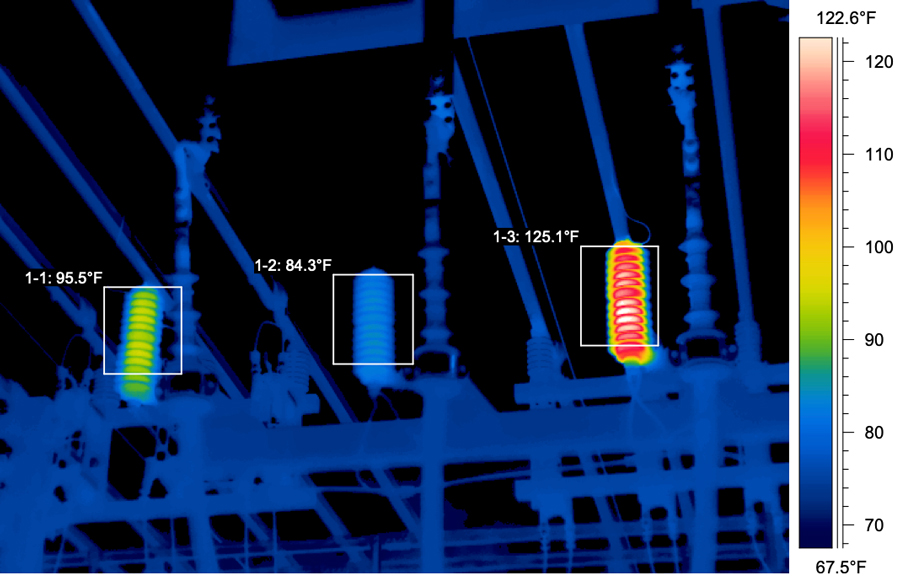
\includegraphics[width=0.75\textwidth]{survey.png}
    \caption{Thermal surveys}
    \label{fig:ts_challenges}
\end{figure}

\subsubsection*{Design \& Implementation of Application}

\paragraph{(i) Data Collection and Annotation:}
\begin{itemize}
    \item \textbf{Thermal Image Acquisition:}  
    Steel, concrete, wood, and composite specimens were heated in a calibrated furnace to target set‐points (200 °C, 400 °C, 600 °C, 800 °C). A FLIR One Pro camera captured images at 5 fps, generating 2 400 labeled frames.
    \item \textbf{Ground‐Truth Logging:}  
    K‐type thermocouples measured actual surface temperatures. Frames with $|\Delta T| > 10\,\mathrm{^{\circ}C}$ from set‐points were discarded to ensure label accuracy.
    \item \textbf{Annotation Pipeline:}  
    Custom scripts embedded material type, emissivity, and timestamp metadata into EXIF tags. A manual validation step confirmed label consistency and removed corrupted images.
\end{itemize}

\paragraph{(ii) Pre‐processing and Augmentation:}
\begin{itemize}
    \item \textbf{Emissivity Correction:}  
    Applied per-material emissivity tables to linearize thermal pixel values.  
    \item \textbf{Filtering and Cropping:}  
    Median filtering (3 × 3) removed sensor noise; center‐crop to 460 × 460 px standardized input dimensions.  
    \item \textbf{Augmentation Strategies:}  
    Domain‐preserving transforms in \texttt{albumentations}: random rotation (±15°), horizontal flip, brightness/contrast jitter (±10 %), Cutout masks (8–14 px), Gaussian blur ($\sigma \le 0.5$). These mitigated overfitting and improved generalization.
\end{itemize}

\paragraph{(iii) Model Development:}
\begin{itemize}
    \item \textbf{ViT Fine‐Tuning:}  
    A ViT‐Base (12 layers, 8 × 8 patch, 768‐dim embedding, 12 heads) pretrained on ImageNet-21k was adapted. Hyper‐parameters: batch size = 32, AdamW ($\beta_1=0.9,\ \beta_2=0.999$), initial LR = 3 × 10$^{-4}$ with cosine annealing, weight decay = 1 × 10$^{-2}$.
    \item \textbf{Baseline CNNs:}  
    ResNet-50 and EfficientNet-B0 were trained from scratch for comparison. Early stopping and learning‐rate schedulers ensured robust convergence.
    \item \textbf{Cross‐Validation and Ablations:}  
    Five‐fold stratified splits assessed macro‐F1 and ROC-AUC. Ablation studies on patch sizes (8 × 8 vs. 16 × 16), augmentation variants, and positional encoding types quantified their impact on performance.
    \item \textbf{Explainability Integration:}  
    Grad-CAM adapted for ViT by backpropagating through the final attention block, generating pixel‐level heatmaps to highlight regions influencing each prediction.
\end{itemize}

\subsubsection*{Backend \& Real‐Time Features}

\paragraph{(i) Technologies Utilized:}
\begin{itemize}
    \item \textbf{Inference Engine:}  
    PyTorch 2.1 for model loading and inference; NVIDIA Apex for mixed‐precision (FP16/FP32) training.
    \item \textbf{Optimization:}  
    TorchScript serialization and TensorRT INT8 quantization reduced model size to ≈80 MB and improved inference speed by ≈28 %.  
    \item \textbf{Microservice:}  
    FastAPI served inference requests; Docker container (≈1.1 GB CUDA image) bundled model, dependencies, and REST endpoints.
    \item \textbf{GUI:}  
    Streamlit provided an interactive interface for single‐image and batch inferences, displaying class labels, confidence scores, and Grad-CAM overlays.
\end{itemize}

\paragraph{(ii) Real‐Time Communication and Logging:}
\begin{itemize}
    \item \textbf{REST Endpoints:}  
    \texttt{/upload}, \texttt{/infer}, \texttt{/heatmap} APIs accepted images in PNG, JPEG, or radiometric TIFF and returned JSON with predicted class and heatmap encoded in base64.
    \item \textbf{Logging and Metrics:}  
    PostgreSQL stored inference logs (timestamp, material, predicted class, confidence). Prometheus metrics tracked P95 latency, GPU utilization, and request throughput.
    \item \textbf{Error Handling:}  
    Graceful error responses for invalid formats, model‐load failures, and inference timeouts, guiding users on corrective actions.
\end{itemize}

\subsection{Proposed Solution}
The proposed solution aims to address thermal inspection challenges by combining fine‐grained ViT classification with a user‐centric interface and edge‐ready deployment:

\begin{itemize}
    \item \textbf{Multi‐Class Thermal Classification:}  
    Automatically categorizes materials into four precise temperature bands (200 °C, 400 °C, 600 °C, 800 °C) with ≥94 % accuracy, facilitating early detection of heat‐induced degradation.
    \item \textbf{Explainable Heatmaps:}  
    Grad-CAM overlays highlight critical thermal regions, enhancing inspector trust and meeting regulatory transparency requirements.
    \item \textbf{Real‐Time Inference:}  
    Sub-350 ms latency on commodity GPUs; CPU fallback <3 s ensures field applicability without high‐end hardware.
    \item \textbf{Edge‐Ready Deployment:}  
    Lightweight TorchScript+TensorRT bundle (≈80 MB) runs on NVIDIA Jetson and x86 platforms, enabling offline operation in remote or cloud‐restricted environments.
    \item \textbf{User Interface:}  
    Streamlit desktop/web app with intuitive controls for uploading images, selecting model versions, and visualizing results. Non‐expert inspectors receive actionable diagnostics in seconds.
\end{itemize}

\subsection{Work Breakdown Structure}
The work structure of ThermoSight is outlined as follows:

\textbf{Phase 1: Data Acquisition \& Preprocessing}
\begin{itemize}
    \item Capture IR images of steel, concrete, wood, and composite specimens at four set-points.
    \item Log ground-truth temperatures with thermocouples; discard outliers ($|\Delta T| > 10\,\mathrm{^{\circ}C}$).
    \item Implement emissivity correction, median filtering, and center-crop to 460 × 460 px.
    \item Develop augmentation scripts (rotation, flip, jitter, Cutout, blur).
    \item Generate stratified 70/15/15 train/validation/test splits.
\end{itemize}

\textbf{Phase 2: Model Development \& Validation}
\begin{itemize}
    \item Train ResNet-50 and EfficientNet-B0 baselines; record accuracy and latency.
    \item Fine-tune ViT-Base with mixed precision; conduct five-fold cross-validation.
    \item Perform ablation studies (patch size, augmentation, encoding).
    \item Integrate and validate Grad-CAM for ViT; verify heatmap alignment with thermocouple hotspots.
\end{itemize}

\textbf{Phase 3: Deployment \& Field Trials}
\begin{itemize}
    \item Export ViT to TorchScript; optimize with TensorRT INT8 quantization.
    \item Build minimal CUDA Docker image bundling FastAPI and Streamlit.
    \item Conduct end-to-end integration tests (upload → inference → heatmap).
    \item Run pilot trials with inspectors; collect feedback on GUI usability and heatmap interpretability.
    \item Refine UI (colormap options, confidence threshold slider) based on field feedback.
    \item Develop user manual, API Swagger spec, and CI/CD pipeline (GitHub Actions).
\end{itemize}

\textbf{Phase 4: Continuous Integration \& Quality Assurance}
\begin{itemize}
    \item Implement CI pipeline: \texttt{pytest} (≥95 % coverage), \texttt{flake8}, \texttt{black}, GPU smoke tests on each PR.
    \item Perform security scans (Trivy) on Docker images; penetration testing of REST endpoints (OWASP ZAP).
    \item Tag semantic versions for reproducible model and API deployments.
\end{itemize}

\subsection{Tools \& Technology}
Following are the tools and technologies employed for the development of ThermoSight:

\begin{itemize}
    \item \textbf{Infrared Cameras:} FLIR One Pro and Seek Thermal Pro for data acquisition; K‐type thermocouples for ground‐truth logging.
    \item \textbf{Deep Learning Frameworks:} PyTorch 2.1, Hugging Face Transformers, \texttt{timm}, NVIDIA Apex for mixed‐precision training.
    \item \textbf{Image Preprocessing Libraries:} \texttt{albumentations} for augmentations; OpenCV for filtering and cropping.
    \item \textbf{Model Optimization:} TorchScript for serialization; NVIDIA TensorRT for INT8 quantization; Docker for containerization.
    \item \textbf{Backend \& API:} FastAPI for RESTful services; Uvicorn for ASGI server; PostgreSQL for logging; Prometheus and Grafana for metrics.
    \item \textbf{User Interface:} Streamlit 1.25 for interactive GUI; PyInstaller for standalone desktop builds.
    \item \textbf{Experiment Tracking:} Weights & Biases 0.21 for hyper‐parameter logging, cross‐validation metrics, and ablation results.
    \item \textbf{Version Control \& CI/CD:} GitHub Actions for automated testing (\texttt{pytest}, \texttt{flake8}, GPU smoke tests) and Docker image builds; Trivy for security scanning.
\end{itemize}
